%
%                  Politecnico di Milano
%
%        Studente: Caravano Andrea
%            A.A.: 2022/2023
%
% Ultima modifica: 04/05/2023
%
%     Descrizione: Prova Finale (Progetto) di Reti Logiche - A.A. 2022/23
%                  Relazione del lavoro svolto
%

\documentclass[a4paper,11pt]{article} % tipo di documento
\usepackage[T1]{fontenc} % codifica dei font
\usepackage[utf8]{inputenc} % lettere accentate da tastiera
\usepackage[english,italian]{babel} % lingua del documento
\usepackage{lipsum} % genera testo fittizio
\usepackage{url} % per scrivere gli indirizzi Internet e/o di riferimento nella pagina

\usepackage[hidelinks]{hyperref} % per modificare il comportamento dei collegamenti ipertestuali (+ leva colore attorno)

\usepackage[margin=0.7in]{geometry} % margine di pagina

\usepackage{graphicx} % per inserire immagini

\usepackage{tikz} % pacchetto per la produzione di diagrammi
\usetikzlibrary{automata, positioning, arrows} % librerie per il tracciamento di ASF/FSM

\usepackage[outputdir=../auxil]{minted} % per colorazione automatica del codice (installare pygments da Homebrew)
% \usepackage{pythonhighlight} % per Python

\setminted{ % si può impostare il linguaggio specifico con \setminted[JSON] ad esempio
    linenos=true,
    breaklines=true,
    encoding=utf8,
    fontsize=\normalsize,
    frame=lines
}

\usepackage{fancyhdr}
\usepackage{textcomp} % per gestione intestazione e piè di pagina

\hypersetup{ % metadati di titolo e autore nel PDF
    pdftitle={Prova Finale di Reti Logiche - A.A. 2022/23},
    pdfauthor={Andrea Caravano}
}

\setlength{\parindent}{0pt} % rimuove l'indentazione del testo

\begin{document}
    \pagestyle{fancy}
    \fancyhead{}\fancyfoot{}
    \fancyhead[L]{\textbf{Prova Finale (Progetto) di Reti Logiche}}
    \fancyhead[R]{Andrea Caravano}
    \fancyfoot[C]{\thepage}

    \title{\textbf{Prova Finale (Progetto) di Reti Logiche}\\Relazione del lavoro svolto}
    \author{Andrea Caravano}
    \date{Anno Accademico 2022--23}
    \maketitle

    \tableofcontents

    \newpage


    \section{Introduzione}\label{sec:introduzione}

    \subsection{Descrizione ad alto livello}\label{subsec:descrizione-ad-alto-livello}
    Nell'ambito della Prova Finale (Progetto) di Reti Logiche, è richiesto lo sviluppo di un componente hardware implementabile su FPGA (dispositivo logico programmabile),
    quali quelle della serie Artix-7 di Xilinx.

    Il software che si richiede di utilizzare per lo sviluppo, simulazione e sintesi (simulata virtualmente) è anch'esso di Xilinx, Vivado.

    \smallskip

    Il componente ha accesso (attraverso segnali opportuni) ad una memoria, che provvede, fornito un indirizzo da 16 bit, ad esporre in uscita i corrispettivi 8 bit di dato,
    parallelamente.

    Esso fa inoltre uso dei segnali principali \texttt{START} e \texttt{W}, caratterizzanti, rispettivamente, la validità della sequenza di bit e la sequenza effettiva,
    suddivisa in \texttt{Identificativo del canale} ($2\ bit$, sempre presenti) e seguiti dall'\texttt{Indirizzo di memoria} ($16\ bit$, al più).

    Se i bit di indirizzo non sono completi, il componente provvede a completarli con dei bit di \texttt{padding}, anticausalmente alla sequenza (in cima).

    \smallskip

    L'identificativo di canale fornito è utilizzato per esporre, su uno dei 4 segnali di uscita (\texttt{$Z_0$}, \texttt{$Z_1$}, \texttt{$Z_2$}, \texttt{$Z_3$}) il dato
    letto dalla memoria all'indirizzo specificato.

    L'elaborazione necessaria avviene entro 20 cicli di clock, con l'attivazione (per un solo ciclo di clock, quello in cui il dato viene esposto) di un segnale \texttt{DONE}, che
    viene disattivato nuovamente al termine.

    Durante questa fase, il componente si “ricorda” dei dati precedentemente esposti sui 4 segnali di uscita (dall'ultimo reset) e, se non sovrascritti dall'ultima lettura, li espone nuovamente.

    Non vi sono verifiche ulteriori da parte del componente relativamente alla violazione della specifica (una sequenza \texttt{W} più corta di 2 bit
    o un indirizzo più lungo di 16 bit).

    \subsection{Un primo esempio}\label{subsec:un-primo-esempio}

    Nell'esempio mostrato, (\hyperref[subsubsec:test-bench-n.-1]{esteso ulteriormente in seguito}), viene prelevato dalla memoria il dato presente all'indirizzo $19$
    (in binario, $10011$) ed esposto sul canale $Z_0$ (identificato da \texttt{00}, in binario).

    In memoria è stato predisposto il valore $134$ (esemplificativo) a tale indirizzo.

    A seguito del segnale di reset, il componente fa uso del seguente schema:

    \medskip

    \begin{tabular}{|c|c|}
        \hline
        \multicolumn{2}{|c|}{\texttt{START} = 1} \\
        \hline
        Identificativo del canale & Indirizzo di memoria \\
        \hline
    \end{tabular}

    \medskip

    Quindi, in questo caso:

    \medskip

    \begin{tabular}{|c|c|}
        \hline
        \multicolumn{2}{|c|}{\texttt{START} = 1} \\
        \hline
        $00$ ($Z_0$) & $10011$ ($19$) \\
        \hline
    \end{tabular}

    \medskip

    Il segnale di \texttt{START} torna dunque a $0$.

    Entro 20 cicli, il componente si occupa di fornire alla memoria l'indirizzo da cui è intenzionato a prelevare il dato e lo preleva, esponendolo sull'uscita corrispettiva
    all'identificativo di cancale richiesto.

    La fase di valorizzazione dei segnali di uscita dura 1 ciclo di clock e segue lo schema seguente:

    \medskip

    \begin{tabular}{|c|c|c|c|}
        \hline
        \multicolumn{4}{|c|}{\texttt{DONE} = 1} \\
        \hline
        $Z_0$ & $Z_1$ & $Z_2$ & $Z_3$ \\
        \hline
        $x$   & $y$   & $z$   & $w$   \\
        \hline
    \end{tabular}

    \medskip

    dove

    $x$ = valore assunto da $Z_0$ l'ultima volta che il segnale di \texttt{DONE} è stato = 1 (0 altrimenti).

    $y$ = valore assunto da $Z_1$ l'ultima volta che il segnale di \texttt{DONE} è stato = 1 (0 altrimenti).

    $z$ = valore assunto da $Z_2$ l'ultima volta che il segnale di \texttt{DONE} è stato = 1 (0 altrimenti).

    $w$ = valore assunto da $Z_3$ l'ultima volta che il segnale di \texttt{DONE} è stato = 1 (0 altrimenti).

    \medskip

    Quindi, nel nostro caso:

    \medskip

    \begin{tabular}{|c|c|c|c|}
        \hline
        \multicolumn{4}{|c|}{\texttt{DONE} = 1} \\
        \hline
        $Z_0$              & $Z_1$          & $Z_2$          & $Z_3$          \\
        \hline
        $10000110$ ($134$) & $00000000$ (0) & $00000000$ (0) & $00000000$ (0) \\
        \hline
    \end{tabular}

    \bigskip

    Viene infine mostrato di seguito lo schema riepilogativo durante l'esposizione del dato (\texttt{DONE} = 1):

    \medskip

    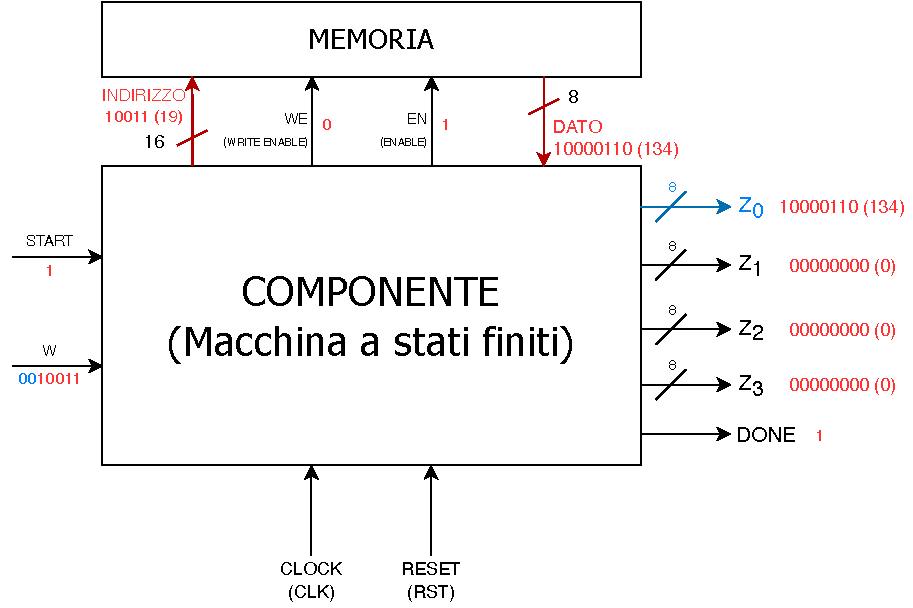
\includegraphics[height=10cm]{../res/disegno-esempio-introduzione}

    \newpage


    \section{Architettura}\label{sec:architettura}

    \subsection{Astrazione}\label{subsec:astrazione}
    L'implementazione astratta del componente è realizzata come mostrato:

    \medskip

    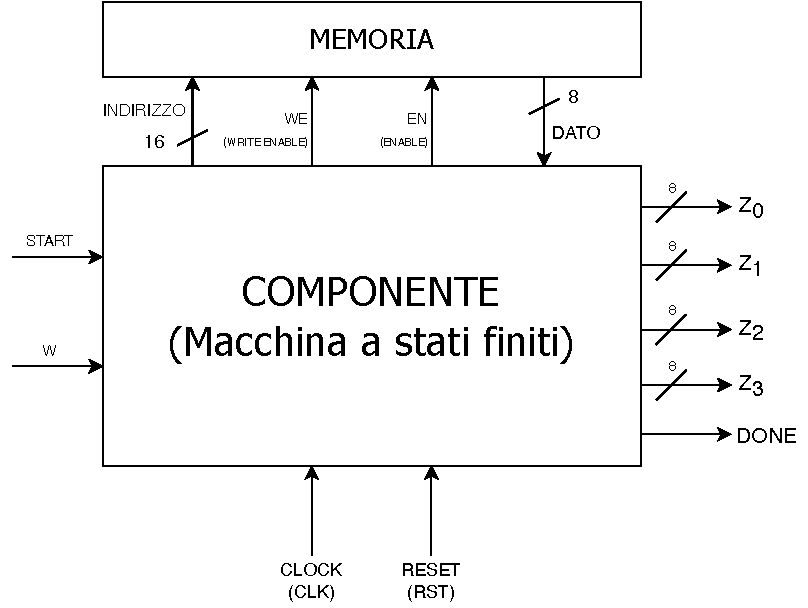
\includegraphics[height=12cm]{../res/disegno-circuito-fsm}

    I cui segnali di riferimento sono:

    \medskip

    \begin{tabular}{|c|c|c|}
        \hline
        Segnale                   & Dimensione ($bit$) & Funzione                                                                  \\
        \hline
        \texttt{CLOCK (CLK)}      & 1                  & Segnale di clock                                                          \\
        \hline
        \texttt{RESET (RST)}      & 1                  & Segnale di reset                                                          \\
        \hline
        \texttt{START}            & 1                  & Delimitatore di validità della sequenza (\texttt{W})                      \\
        \hline
        \texttt{W}                & 1                  & Sequenza aggregata effettiva, suddivisa in                                \\
        &                    & \texttt{Identificativo del canale} e \texttt{Indirizzo di memoria}        \\
        \hline
        Indirizzo                 & 16                 & Trasmesso alla memoria, derivante dalla Sequenza aggregata                \\
        &                    & \hyperref[subsec:descrizione-ad-alto-livello]{(eventualmente completato)} \\
        \hline
        \texttt{Write Enable(WE)} & 1                  & Attivo quando è richiesto di scrivere dati in memoria.                    \\
        &                    & Nell'ambito di questo progetto, è sempre disattivo (impostato a $0$).     \\
        \hline
        \texttt{Enable (EN)}      & 1                  & Attivo quando è richiesto in generale l'uso della memoria.                \\
        &                    & Nell'ambito di questo progetto, è sempre attivo (impostato a $1$).        \\
        \hline
        Dato                      & 8                  & Letto dalla memoria, in corrispondenza dell'indirizzo indicato.           \\
        &                    & Esso viene reso effettivamente disponibile dopo un ciclo di clock         \\
        &                    & rispetto all'indicazione alla memoria dell'indirizzo.                     \\
        \hline
        $Z_0$                     & 8                  & Canale di uscita corrispondente all'identificativo di canale \texttt{00}  \\
        \hline
        $Z_1$                     & 8                  & Canale di uscita corrispondente all'identificativo di canale \texttt{01}  \\
        \hline
        $Z_2$                     & 8                  & Canale di uscita corrispondente all'identificativo di canale \texttt{10}  \\
        \hline
        $Z_3$                     & 8                  & Canale di uscita corrispondente all'identificativo di canale \texttt{11}  \\
        \hline
        \texttt{DONE}             & 1                  & Attivo per un ciclo di clock durante la fase di esposizione del dato      \\
        &                    & trovato in memoria all'indirizzo fornito (ed eventualmente degli          \\
        &                    & ultimi valori esposti precedentemente in questa fase)                     \\
        \hline
    \end{tabular}

    \newpage

    \subsection{Macchina a stati finiti}\label{subsec:macchina-a-stati-finiti}

    La macchina a stati finiti fa uso del seguente diagramma di stato:

    \medskip

    % Configurazione libreria Tikzset
    \tikzset{
        ->, % makes the edges directed
        >=stealth', % makes the arrow heads bold
        node distance=5cm, % specifies the minimum distance between two nodes. Change if necessary.
        every state/.style={thick, fill=gray!10, minimum size=2.7cm}, % sets the properties for each ’state’ node
        initial text=$$, % sets the text that appears on the start arrow
    }

    % Diagramma FSM
    \scalebox{0.9}
    {
        \begin{tikzpicture}
            \node[state, initial] (q1) {\tiny{$WAIT\_START$}};
            \node[state, right of=q1] (q2) {\tiny{$READ\_FIRST$}};
            \node[state, right of=q2] (q3) {\tiny{$READ\_SECOND$}};
            \node[state, right of=q3] (q4) {\tiny{$READ\_ADDR$}};
            \node[state, below of=q3] (q5) {\tiny{$WAIT\_DATA$}};
            \node[state, below of=q2] (q6) {\tiny{$READ\_AND\_OUT$}};

            \draw
            (q1) edge[loop above] node{\scriptsize{START=0}} (q1)
            (q1) edge[above] node{\scriptsize{START=1}} (q2)
            (q2) edge[above] node{\scriptsize{START=1}} (q3)
            (q3) edge[above] node{\scriptsize{START=1}} (q4)
            (q4) edge[loop above] node{\scriptsize{START=1}} (q4)
            (q3) edge[below, left=0.5] node{\scriptsize{START=0}} (q5)
            (q4) edge[below, bend left, right=0.5] node{\scriptsize{START=0}} (q5)
            (q5) edge[above] node{} (q6)
            (q6) edge[below, bend left] node{} (q1);
        \end{tikzpicture}
    }

    \medskip

    Implementati come descritto nel seguito.

    \subsubsection{\texttt{WAIT\_START}}

    Stato iniziale del ciclo, i segnali di \texttt{DONE}, i canali di uscita, il buffer dell'indirizzo e il contatore della relativa lunghezza vengono tutti reimpostati
    al valore predefinito ($0$).

    Tale stato viene mantenuto finché il segnale di \texttt{START} (delimitatore di validità della sequenza) rimane $0$.
    In caso contrario, si prosegue nella lettura del primo bit componente l'\texttt{Identificativo del canale} di uscita.

    \subsubsection{\texttt{READ\_FIRST}}

    In corrispondenza dell'attivazione del segnale di \texttt{START}, viene letto il primo bit che compone l'\texttt{Identificativo del canale} di uscita.

    \subsubsection{\texttt{READ\_SECOND}}

    Viene letto il secondo bit componente l'\texttt{Identificativo del canale} di uscita.

    Come da specifica, non sono previste transizioni nel caso in cui i segnali ricevuti non rispettino le indicazioni sulla durata minima (o massima) della sequenza \texttt{W},
    che si tradurrebbero comunque nella permanenza in uno stato di errore.
    Si noti inoltre che l'indirizzo può essere vuoto ($0\ bit$).

    \subsubsection{\texttt{READ\_ADDR}}

    Fino a quando il segnale di \texttt{START} rimane a $1$ (indicante la validità della sequenza \texttt{W}), vengono memorizzati i bit che compongono l'indirizzo in un buffer
    temporaneo, seguendo l'ordine di arrivo.

    In questa fase non vengono effettuate traslazioni dell'indirizzo per eventuali \texttt{bit di padding}, che si rimandano invece alla successiva.

    \subsubsection{\texttt{WAIT\_DATA}}

    Stato di attesa del ciclo di clock necessario alla memoria per esporre il dato sul corrispondente segnale.

    L'indirizzo fornito è comprensivo di eventuali \texttt{bit di padding} necessari per completare i $16$ richiesti.

    \subsubsection{\texttt{READ\_AND\_OUT}}

    Fase in cui il segnale \texttt{DONE} è attivo.

    Il dato trovato in memoria all'indirizzo specificato viene esposto sul canale scelto, gli altri canali (solo in questa fase) espongono l'ultimo valore esposto in questa
    fase, 0 altrimenti.

    Le uscite seguono dunque lo schema esposto \hyperref[subsec:un-primo-esempio]{nell'esempio introduttivo}.

    Al termine, il segnale \texttt{DONE} viene posto nuovamente a $0$ e il componente ritorna nella fase iniziale (\texttt{WAIT\_START}).


    \section{Risultati sperimentali}\label{sec:risultati-sperimentali}
    La specifica del componente è stata implementata in VHDL su Xilinx Vivado 2018.3.1, attraverso la piattaforma di Virtual Desktop Citrix offerta dal Politecnico.

    Sempre in Vivado sono state realizzate varie configurazioni di test bench, come esposto nel seguito.

    \subsection{Sintesi}\label{subsec:sintesi}
    Di seguito, viene riportato il report della sintesi, in cui viene mostrato il numero di registri utilizzato.

    Si noti inoltre, come raccomandato a lezione, l'assenza di Latch, che potrebbero indicare problemi nella gestione dei segnali del componente.

    \medskip

    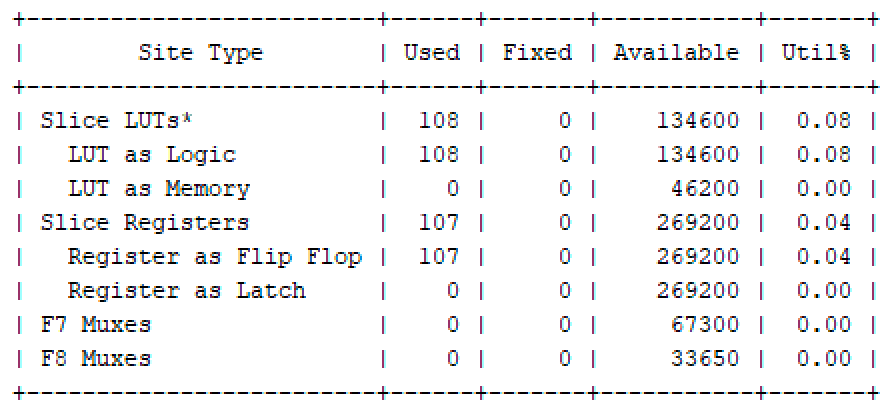
\includegraphics[height=4cm]{../res/report-registri}

    Inoltre, il componente non presenta problemi legati al timing, come mostrato:
    \smallskip

    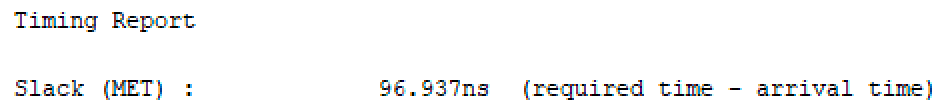
\includegraphics[height=1.3cm]{../res/report-timing}

    Dalla sintesi, completata con successo, deriva lo schema seguente:

    \medskip

    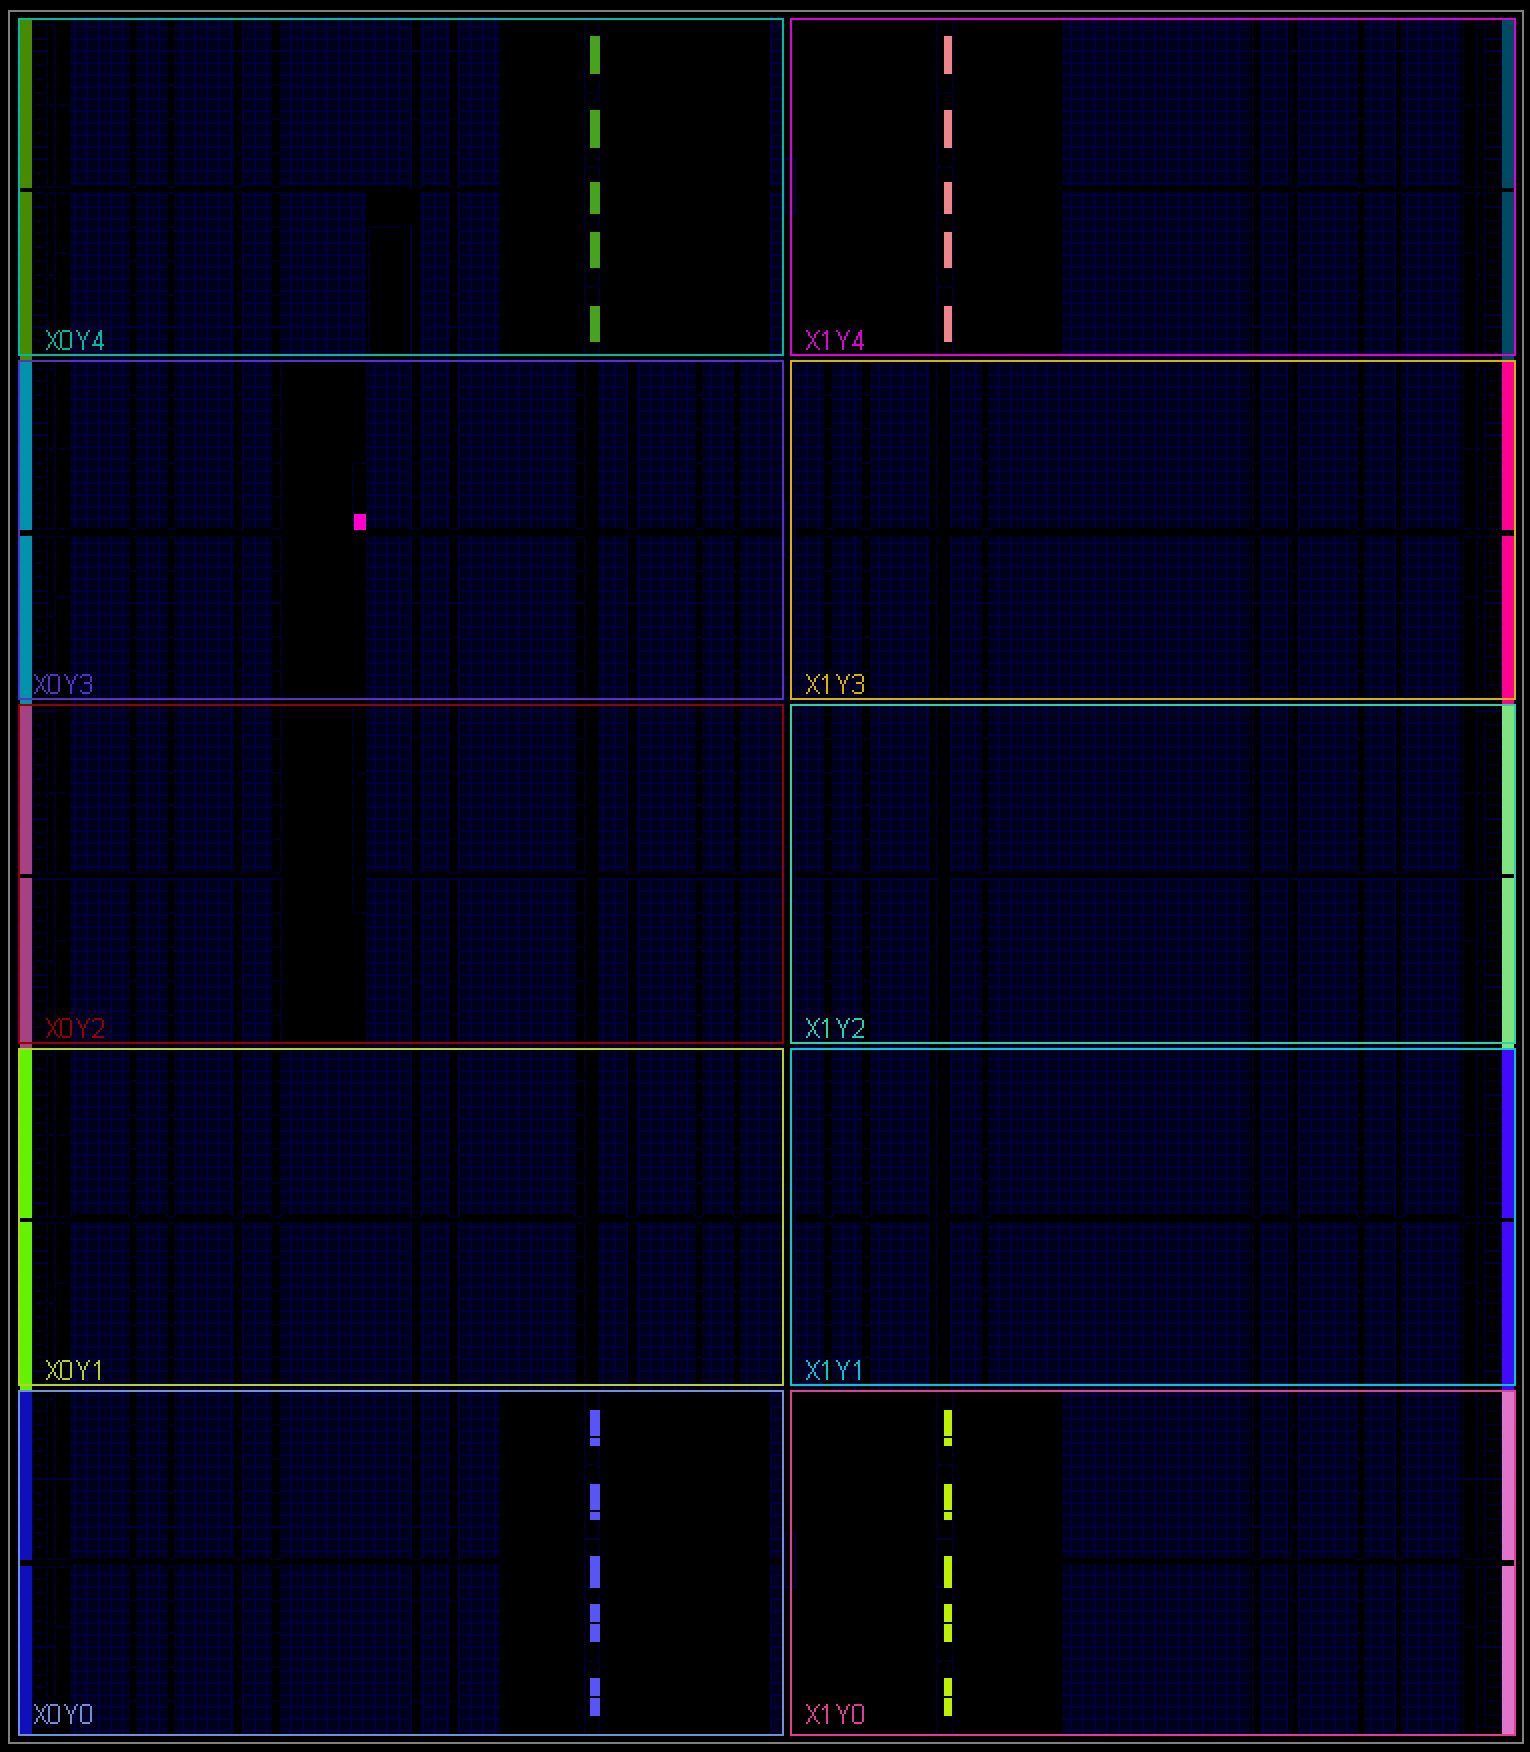
\includegraphics[height=10cm]{../res/design-sintesi}

    \newpage

    \subsection{Simulazioni}\label{subsec:simulazioni}
    Sono state realizzate diverse configurazioni di casi di test, a partire dal test bench di riferimento fornito.

    Nel seguito, ne vengono mostrati alcuni esempi.

    \subsubsection{Test bench n. 1: esempio introduttivo}\label{subsubsec:test-bench-n.-1}
    Implementa l'\hyperref[subsec:un-primo-esempio]{esempio introduttivo}.

    In particolare, a seguito del segnale di reset, ci si aspetta, a seguire i due casi di test iniziali, il primo introdotto:

    \bigskip

    \begin{tabular}{|c|c|}
        \hline
        \multicolumn{2}{|c|}{\texttt{START} = 1} \\
        \hline
        $00$ ($Z_0$) & $10011$ ($19$) \\
        \hline
    \end{tabular}

    \medskip

    \begin{tabular}{|c|c|c|c|}
        \hline
        \multicolumn{4}{|c|}{\texttt{DONE} = 1} \\
        \hline
        $Z_0$              & $Z_1$           & $Z_2$            & $Z_3$          \\
        \hline
        $10000110$ ($134$) & $01011000$ (88) & $10100010$ (162) & $00000000$ (0) \\
        \hline
    \end{tabular}

    \bigskip

    Che corrisponde alla seguente combinazione di segnali:

    \begin{minted}{VHDL}
SIGNAL scenario_rst : unsigned(0 TO SCENARIOLENGTH - 1)     := "00110" & "000" & "00000000000000000000" & "0000000" & "00000000000000000000" & "0000000";
SIGNAL scenario_start : unsigned(0 TO SCENARIOLENGTH - 1)   := "00000"
                         & "111" & "00000000000000000000"
                         & "1111100" & "00000000000000000000"
                         & "1111111";
SIGNAL scenario_w : unsigned(0 TO SCENARIOLENGTH - 1)       := "00000"
                         & "101" & "00000000000000000000"
                         & "0111000" & "00000000000000000000"
                         & "0010011";
    \end{minted}

    E con memoria istanziata:

    \begin{minted}{VHDL}
TYPE ram_type IS ARRAY (65535 DOWNTO 0) OF STD_LOGIC_VECTOR(7 DOWNTO 0);
SIGNAL RAM : ram_type := (  0 => STD_LOGIC_VECTOR(to_unsigned(2, 8)),
                            1 => STD_LOGIC_VECTOR(to_unsigned(162, 8)),
                            2 => STD_LOGIC_VECTOR(to_unsigned(75, 8)),
                            3 => STD_LOGIC_VECTOR(to_unsigned(175, 8)),
                            6 => STD_LOGIC_VECTOR(to_unsigned(88, 8)),
                            19 => STD_LOGIC_VECTOR(to_unsigned(134, 8)), -- aggiunto il valore 134 all'indirizzo 19
                            OTHERS => "00000000"-- (OTHERS => '0')
                         );
    \end{minted}

    \newpage

    L'esecuzione porta dunque al risultato atteso:
    \smallskip

    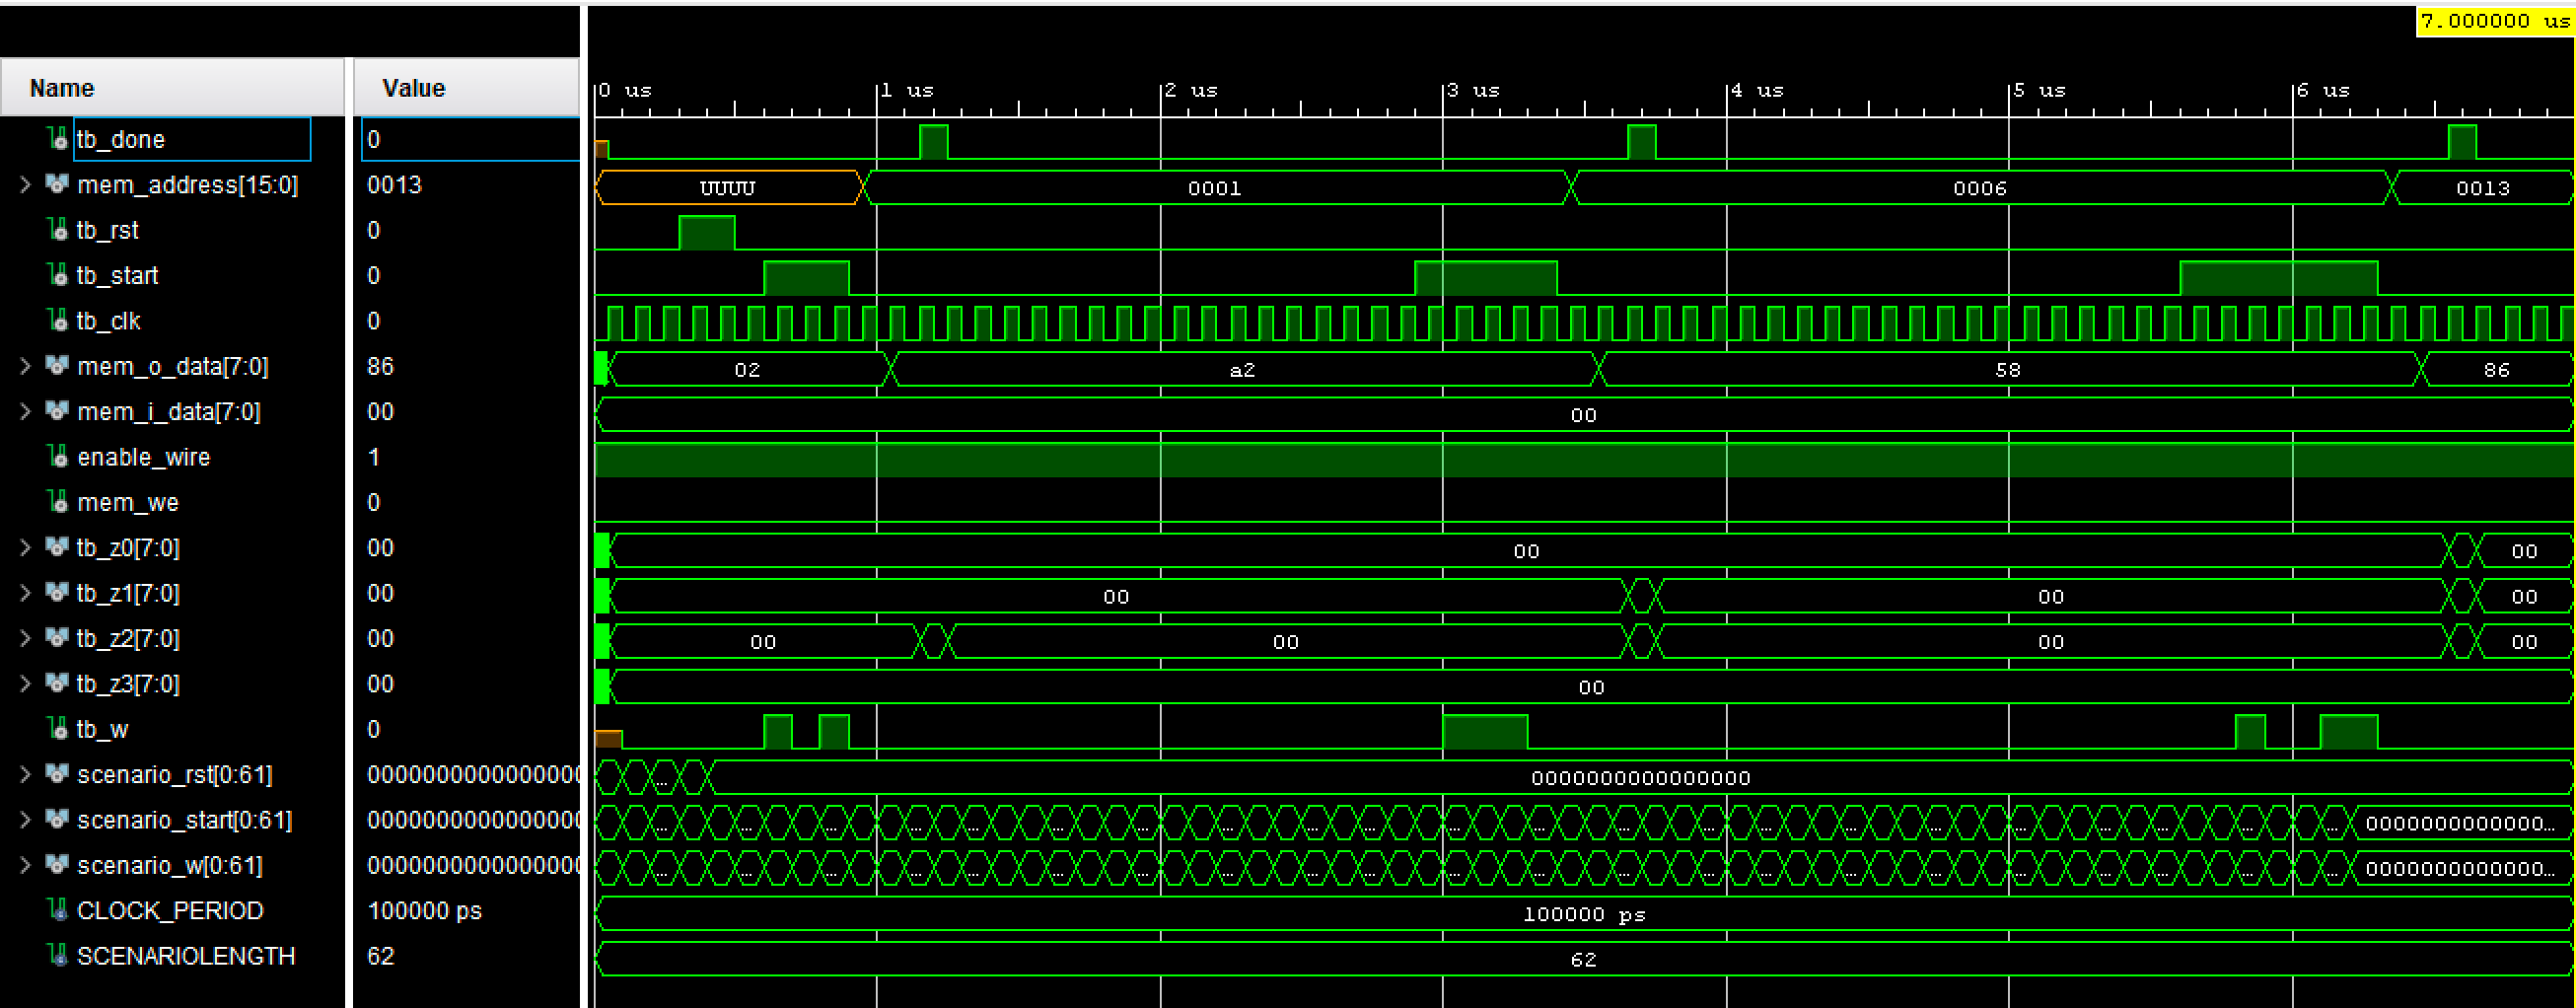
\includegraphics[height=7cm]{../res/tb-1}

    \subsubsection{Test bench n. 2: indirizzo vuoto e sovrascrittura}
    Si testa ora la capacità del componente di reagire correttamente ad un indirizzo vuoto ($0\ bit$).

    Ci si aspetta esso corrisponda all'indirizzo 0 di memoria, presso cui è stato posto il valore di test $135$.

    Si sceglie inoltre di utilizzare il canale \texttt{10} ($Z_2$), verificando anche la corretta sovrascrittura del valore precedente ($162$).

    Quindi, ci si aspetta che la nuova sequenza sia:
    \medskip

    \begin{tabular}{|c|c|}
        \hline
        \multicolumn{2}{|c|}{\texttt{START} = 1} \\
        \hline
        $10$ ($Z_2$) & \textblank \  ($0$) \\
        \hline
    \end{tabular}

    \medskip

    \begin{tabular}{|c|c|c|c|}
        \hline
        \multicolumn{4}{|c|}{\texttt{DONE} = 1} \\
        \hline
        $Z_0$              & $Z_1$           & $Z_2$            & $Z_3$          \\
        \hline
        $10000110$ ($134$) & $01011000$ (88) & $10000111$ (135) & $00000000$ (0) \\
        \hline
    \end{tabular}

    \bigskip

    Che corrisponde alla seguente combinazione di segnali:

    \begin{minted}{VHDL}
SIGNAL scenario_rst : unsigned(0 TO SCENARIOLENGTH - 1)     := "00110" & "000" & "00000000000000000000" & "0000000" & "00000000000000000000" & "0000000" & "00000000000000000000" & "00";
SIGNAL scenario_start : unsigned(0 TO SCENARIOLENGTH - 1)   := "00000"
                         & "111" & "00000000000000000000"
                         & "1111100" & "00000000000000000000"
                         & "1111111" & "00000000000000000000"
                         & "11";
SIGNAL scenario_w : unsigned(0 TO SCENARIOLENGTH - 1)       := "00000"
                         & "101" & "00000000000000000000"
                         & "0111000" & "00000000000000000000"
                         & "0010011" & "00000000000000000000"
                         & "10";
    \end{minted}

    \newpage

    E con memoria istanziata:

    \begin{minted}{VHDL}
TYPE ram_type IS ARRAY (65535 DOWNTO 0) OF STD_LOGIC_VECTOR(7 DOWNTO 0);
SIGNAL RAM : ram_type := (  0 => STD_LOGIC_VECTOR(to_unsigned(135, 8)), -- posto in memoria 135 all'indirizzo 0
                            1 => STD_LOGIC_VECTOR(to_unsigned(162, 8)),
                            2 => STD_LOGIC_VECTOR(to_unsigned(75, 8)),
                            3 => STD_LOGIC_VECTOR(to_unsigned(175, 8)),
                            6 => STD_LOGIC_VECTOR(to_unsigned(88, 8)),
                            19 => STD_LOGIC_VECTOR(to_unsigned(134, 8)),
                            OTHERS => "00000000"-- (OTHERS => '0')
                         );
    \end{minted}

    L'esecuzione porta dunque al risultato atteso:
    \smallskip

    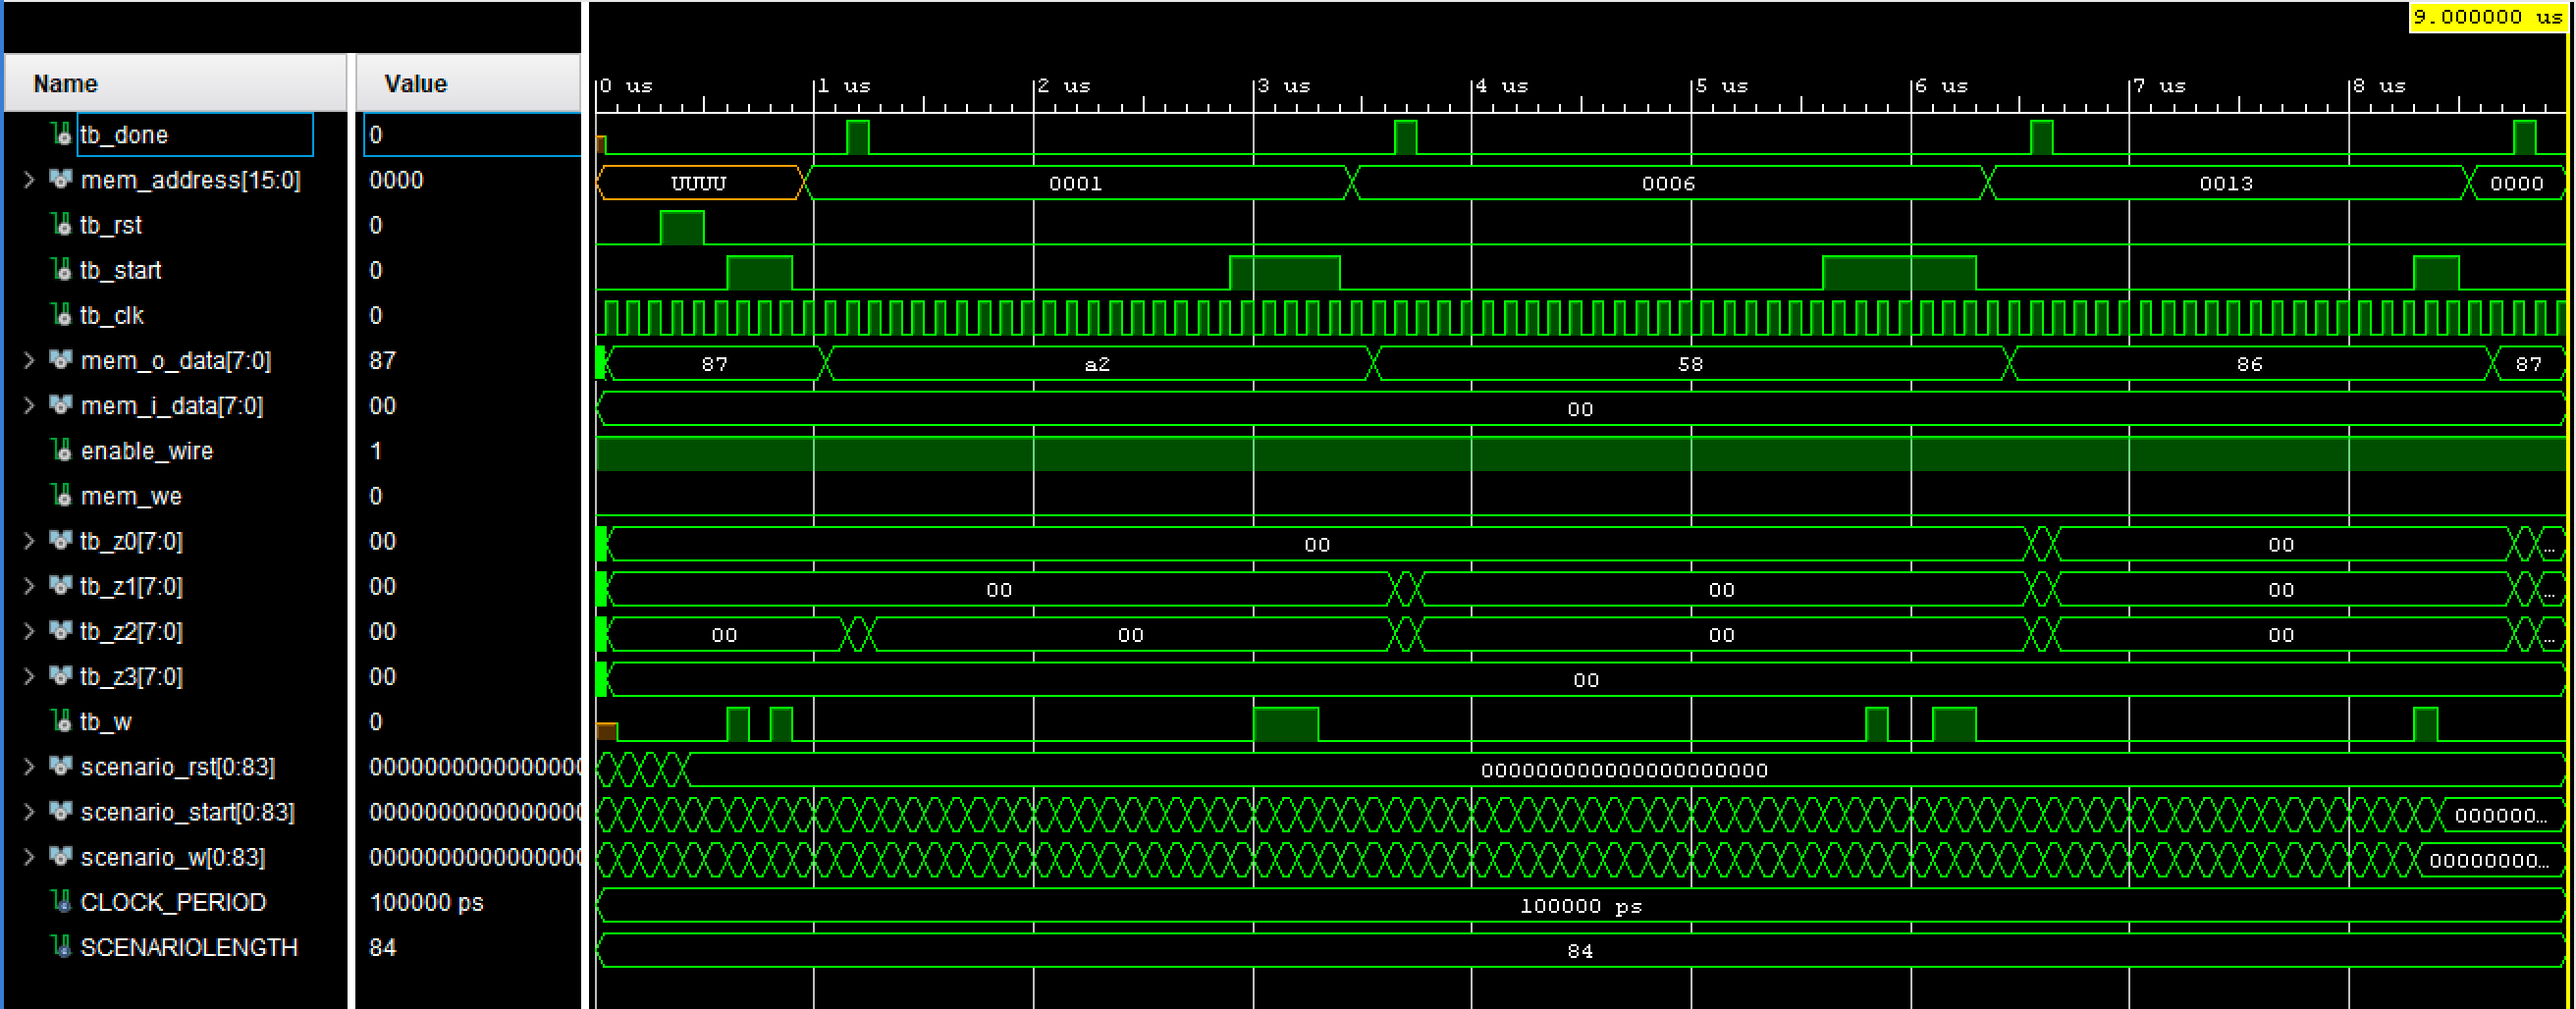
\includegraphics[height=7cm]{../res/tb-2}

    \subsubsection{Test bench n. 3: indirizzo completo e reset}
    Si testa ora la capacità del componente di reagire correttamente ad un indirizzo completo ($16\ bit$).

    Ci si aspetta esso corrisponda all'indirizzo $1000100111111011$ ($35323$) di memoria, presso cui è stato posto il valore di test $142$.

    Si sceglie di utilizzare il canale \texttt{11} ($Z_3$).

    Si noti che l'indirizzo scelto è volutamente non simmetrico o palindromo.

    Prima di procedere, tuttavia, si testa anche l'abilità del componente di reagire correttamente ad un secondo reset, antecedente la lettura di quest'ultima sequenza.

    Quindi, ci si aspetta che la nuova sequenza sia:
    \medskip

    \begin{tabular}{|c|c|}
        \hline
        \multicolumn{2}{|c|}{\texttt{START} = 1} \\
        \hline
        $11$ ($Z_3$) & $1000100111111011$ ($35323$) \\
        \hline
    \end{tabular}

    \medskip

    Prima del reset, ci si aspetta sui canali di uscita:
    \medskip

    \begin{tabular}{|c|c|c|c|}
        \hline
        \multicolumn{4}{|c|}{\texttt{DONE} = 1} \\
        \hline
        $Z_0$              & $Z_1$           & $Z_2$            & $Z_3$          \\
        \hline
        $10000110$ ($134$) & $01011000$ (88) & $10000111$ (135) & $00000000$ (0) \\
        \hline
    \end{tabular}

    \medskip

    A seguire il reset, invece:
    \medskip

    \begin{tabular}{|c|c|c|c|}
        \hline
        \multicolumn{4}{|c|}{\texttt{DONE} = 1} \\
        \hline
        $Z_0$            & $Z_1$            & $Z_2$            & $Z_3$              \\
        \hline
        $00000000$ ($0$) & $00000000$ ($0$) & $00000000$ ($0$) & $10001110$ ($142$) \\
        \hline
    \end{tabular}

    \newpage

    Che corrisponde alla seguente combinazione di segnali:

    \begin{minted}{VHDL}
SIGNAL scenario_rst : unsigned(0 TO SCENARIOLENGTH - 1)     := "00110"
                      & "000" & "00000000000000000000"
                      & "0000000" & "00000000000000000000"
                      & "0000000" & "00000000000000000000"
                      & "00" & "00000000000000000000"
                      & "1" -- reset
                      & "000000000000000000";
SIGNAL scenario_start : unsigned(0 TO SCENARIOLENGTH - 1)   := "00000"
                      & "111" & "00000000000000000000"
                      & "1111100" & "00000000000000000000"
                      & "1111111" & "00000000000000000000"
                      & "11" & "00000000000000000000"
                      & "0"
                      & "111111111111111111";
SIGNAL scenario_w : unsigned(0 TO SCENARIOLENGTH - 1)       := "00000"
                      & "101" & "00000000000000000000"
                      & "0111000" & "00000000000000000000"
                      & "0010011" & "00000000000000000000"
                      & "10" & "00000000000000000000"
                      & "0"
                      & "111000100111111011";
    \end{minted}

    E con memoria istanziata:

    \begin{minted}{VHDL}
TYPE ram_type IS ARRAY (65535 DOWNTO 0) OF STD_LOGIC_VECTOR(7 DOWNTO 0);
SIGNAL RAM : ram_type := (  0 => STD_LOGIC_VECTOR(to_unsigned(135, 8)),
                                1 => STD_LOGIC_VECTOR(to_unsigned(162, 8)),
                                2 => STD_LOGIC_VECTOR(to_unsigned(75, 8)),
                                3 => STD_LOGIC_VECTOR(to_unsigned(175, 8)),
                                6 => STD_LOGIC_VECTOR(to_unsigned(88, 8)),
                                19 => STD_LOGIC_VECTOR(to_unsigned(134, 8)),
                                35323 => STD_LOGIC_VECTOR(to_unsigned(142, 8)), -- posto 142 in memoria all'indirizzo pieno
                                OTHERS => "00000000"-- (OTHERS => '0')
                            );
    \end{minted}

    L'esecuzione porta dunque al risultato atteso:
    \smallskip

    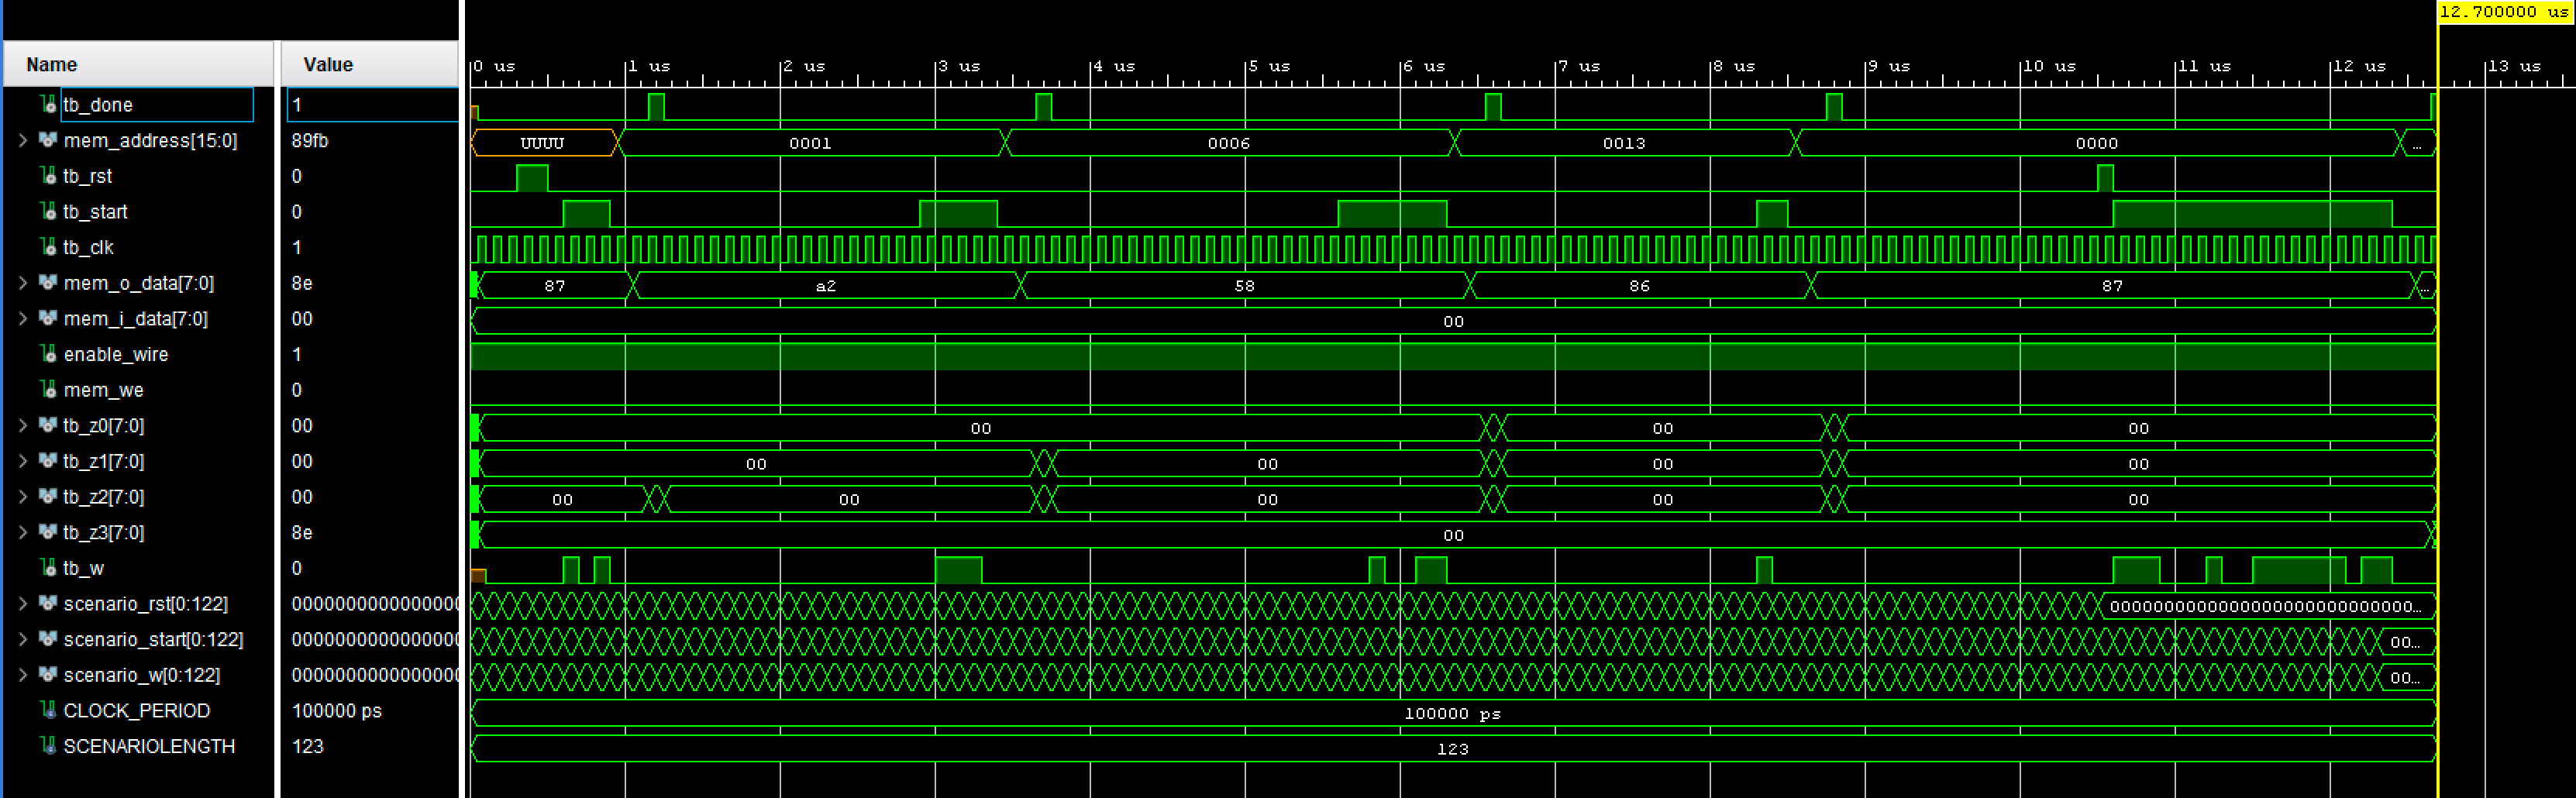
\includegraphics[height=5.5cm]{../res/tb-3}

    \newpage

    \subsubsection{Test bench n. 4: combinazioni e reset multipli}
    Quest'ultimo test bench (come i precedenti) è cumulativo di tutti i test fino ad ora svolti e aggiunge un doppio reset, a valle del quale avviene
    un'ultimo tentativo di lettura in memoria.

    Si tenta, infine, di leggere da un indirizzo di memoria presso il quale è posto il dato convenzionale di default ($0$).

    Per primo, si sceglie di utilizzare come indirizzo in memoria \texttt{1111101000} ($1000$), presso cui ci si aspetta di trovare il valore di default $0$.

    Il canale di uscita scelto è \texttt{01} ($Z_1$).

    Terminata tale lettura, si sceglie di utilizzare come indirizzo in memoria \texttt{10} ($2$), che è rimasto fino ad ora inutilizzato e a cui è posto il valore $75$.

    Il canale di uscita è nuovamente $Z_1$, presso cui si aspetta ora di trovare $75$.

    Infine, viene effettuato un altro reset, a valle del quale si sceglie di utilizzare come indirizzo in memoria \texttt{11} ($3$), che è rimasto fino ad ora inutilizzato e a cui è posto il valore $175$.

    Il canale di uscita scelto per quest'ultima lettura è \texttt{10} ($Z_2$).

    Ci si aspetta gli altri canali espongano ora valore nullo.

    Quindi, ci si aspetta che la nuova sequenza sia:
    \medskip

    \begin{tabular}{|c|c|}
        \hline
        \multicolumn{2}{|c|}{\texttt{START} = 1} \\
        \hline
        $01$ ($Z_1$) & $1111101000$ ($1000$) \\
        \hline
    \end{tabular}

    \medskip

    Seguito da:

    \smallskip

    \begin{tabular}{|c|c|}
        \hline
        \multicolumn{2}{|c|}{\texttt{START} = 1} \\
        \hline
        $01$ ($Z_1$) & $10$ ($2$) \\
        \hline
    \end{tabular}

    \medskip

    A seguire l'ultimo reset:
    \smallskip

    \begin{tabular}{|c|c|}
        \hline
        \multicolumn{2}{|c|}{\texttt{START} = 1} \\
        \hline
        $10$ ($Z_2$) & $11$ ($3$) \\
        \hline
    \end{tabular}

    \medskip

    Sulle uscite, inizialmente:
    \medskip

    \begin{tabular}{|c|c|c|c|}
        \hline
        \multicolumn{4}{|c|}{\texttt{DONE} = 1} \\
        \hline
        $Z_0$            & $Z_1$            & $Z_2$            & $Z_3$              \\
        \hline
        $00000000$ ($0$) & $00000000$ ($0$) & $00000000$ ($0$) & $10001110$ ($142$) \\
        \hline
    \end{tabular}

    \medskip

    Si noti che in $Z_1$ ci si aspetta ancora di trovare 0, perché anche in memoria si trova il valore 0.

    Successivamente:
    \medskip

    \begin{tabular}{|c|c|c|c|}
        \hline
        \multicolumn{4}{|c|}{\texttt{DONE} = 1} \\
        \hline
        $Z_0$            & $Z_1$             & $Z_2$            & $Z_3$              \\
        \hline
        $00000000$ ($0$) & $01001011$ ($75$) & $00000000$ ($0$) & $10001110$ ($142$) \\
        \hline
    \end{tabular}

    \medskip

    In seguito all'ultimo reset, infine:

    \medskip

    \begin{tabular}{|c|c|c|c|}
        \hline
        \multicolumn{4}{|c|}{\texttt{DONE} = 1} \\
        \hline
        $Z_0$            & $Z_1$            & $Z_2$              & $Z_3$            \\
        \hline
        $00000000$ ($0$) & $00000000$ ($0$) & $10101111$ ($175$) & $00000000$ ($0$) \\
        \hline
    \end{tabular}

    \bigskip

    Che corrisponde alla seguente combinazione di segnali:

    \begin{minted}{VHDL}
SIGNAL scenario_rst : unsigned(0 TO SCENARIOLENGTH - 1)     := "00110"
                      & "000" & "00000000000000000000"
                      & "0000000" & "00000000000000000000"
                      & "0000000" & "00000000000000000000"
                      & "00" & "00000000000000000000"
                      & "1" -- reset
                      & "000000000000000000" & "00000000000000000000"
                      & "00000000000" & "00000000000000000000"
                      & "0000" & "00000000000000000000"
                      & "1" -- ulteriore reset
                      & "0000";
    \end{minted}
    \begin{minted}{VHDL}
SIGNAL scenario_start : unsigned(0 TO SCENARIOLENGTH - 1)   := "00000"
                        & "111" & "00000000000000000000"
                        & "1111100" & "00000000000000000000"
                        & "1111111" & "00000000000000000000"
                        & "11" & "00000000000000000000"
                        & "0"
                        & "111111111111111111" & "00000000000000000000"
                        & "11111111111" & "00000000000000000000"
                        & "1111" & "00000000000000000000"
                        & "0"
                        & "1111";
SIGNAL scenario_w : unsigned(0 TO SCENARIOLENGTH - 1)       := "00000"
                        & "101" & "00000000000000000000"
                        & "0111000" & "00000000000000000000"
                        & "0010011" & "00000000000000000000"
                        & "10" & "00000000000000000000"
                        & "0"
                        & "111000100111111011" & "00000000000000000000"
                        & "01111110100" & "00000000000000000000"
                        & "0110" & "00000000000000000000"
                        & "0"
                        & "1011";
    \end{minted}

    E con memoria istanziata:

    \begin{minted}{VHDL}
TYPE ram_type IS ARRAY (65535 DOWNTO 0) OF STD_LOGIC_VECTOR(7 DOWNTO 0);
SIGNAL RAM : ram_type := (  0 => STD_LOGIC_VECTOR(to_unsigned(135, 8)),
                                1 => STD_LOGIC_VECTOR(to_unsigned(162, 8)),
                                2 => STD_LOGIC_VECTOR(to_unsigned(75, 8)), -- valore utilizzato per la lettura
                                3 => STD_LOGIC_VECTOR(to_unsigned(175, 8)), -- valore utilizzato per la lettura
                                6 => STD_LOGIC_VECTOR(to_unsigned(88, 8)),
                                19 => STD_LOGIC_VECTOR(to_unsigned(134, 8)),
                                35323 => STD_LOGIC_VECTOR(to_unsigned(142, 8)),
                                OTHERS => "00000000"-- (OTHERS => '0')
                            );
    \end{minted}

    L'esecuzione porta dunque al risultato atteso:
    \smallskip

    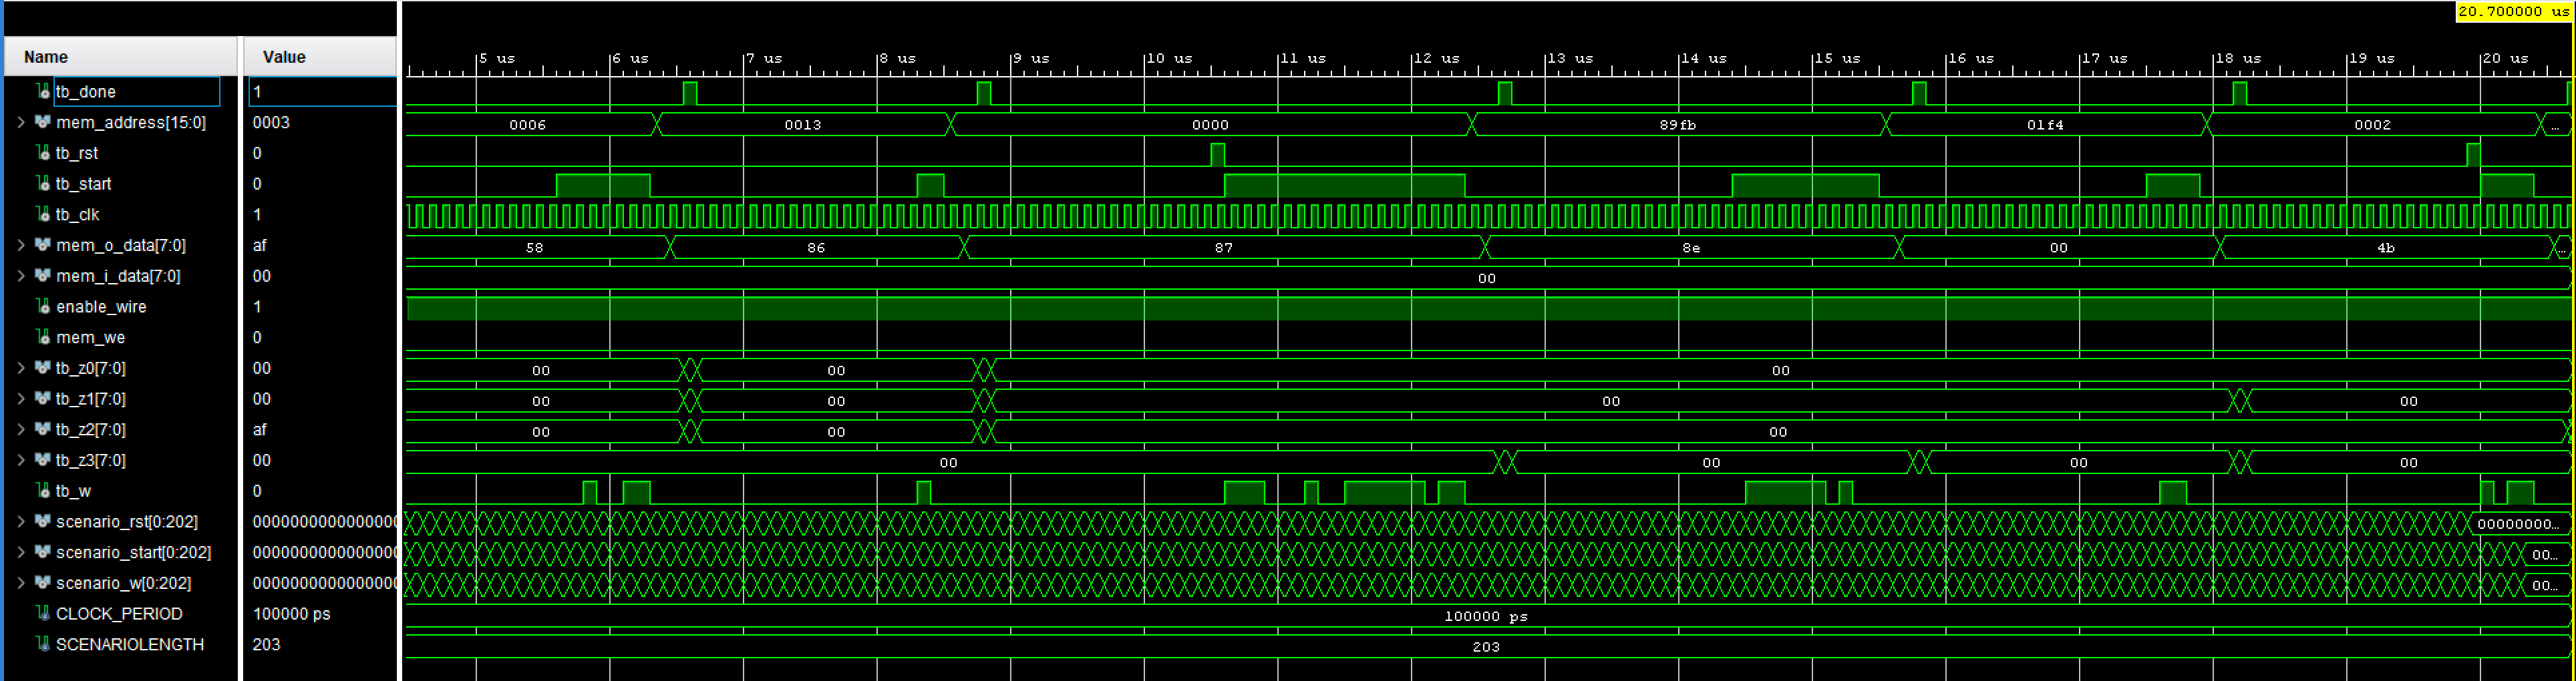
\includegraphics[height=5cm]{../res/tb-4}

    \newpage


    \section{Conclusioni}\label{sec:conclusioni}
    I test bench utilizzati durante lo sviluppo e le fasi di testing, anche post-sintesi, pongono le basi sulle tecniche esposte nel capitolo precedente.

    \bigskip

    Scopo della Prova Finale è dunque stata la gestione del progetto completo di un componente effettivamente implementabile su una FPGA reale Xilinx,
    grazie a Vivado stesso.

    Oltre alle fasi di comprensione ed esemplificazione della specifica si sono dunque utilizzati i paradigmi approfonditi a lezione per realizzare concretamente
    l'implementazione di una macchina a stati finiti (che trova infatti applicazione in un numero sconfinato di applicazioni professionali).

    Si è inoltre svolta una fase approfondita di testing, naturalmente derivante dalle indicazioni della specifica e dei docenti, al fine di consolidare la comprensione e
    l'idoneità dell'implementazione nei confronti della specifica.
\end{document}